\documentclass[conference]{IEEEtran}
\usepackage[utf8]{inputenc}
\usepackage{amsmath,amssymb,graphicx,booktabs}

\usepackage[hidelinks,unicode,pdftitle={Replicating Validation-Selected Weight Interpolation on SmolLM2-360M Base and Instruct: ARC, HellaSwag and WinoGrande},pdfauthor={Dheiver Francisco Santos},pdfkeywords={model merging, weight interpolation, task vectors, SmolLM2, replication, negative result},pdfsubject={Preprint, Figshare, doi:10.6084/m9.figshare.35014000}]{hyperref}
\begin{document}

\title{Replicating Validation-Selected Weight Interpolation on SmolLM2-360M Base and Instruct: ARC, HellaSwag and WinoGrande}

\author{\IEEEauthorblockN{Dheiver Francisco Santos, PhD}
\IEEEauthorblockA{Independent Researcher\\
Maceió, Alagoas, Brazil\\
ORCID: https://orcid.org/0000-0002-8599-9436\\
Preprint, Figshare, 2026, \href{https://doi.org/10.6084/m9.figshare.35014000}{doi:10.6084/m9.figshare.35014000}, CC BY 4.0}}

\maketitle

\begin{abstract}
Selecting an interpolation coefficient between a base language model and its instruct sibling is often presented as a free improvement over both. We replicate a pre-registered test of this claim on SmolLM2-360M and its instruct version, using the same protocol as for Qwen2.5-0.5B with a coarser six-point grid, selection on 300 validation items per task, and 3{,}967 disjoint test items. The selected $t^\ast=0.2$ scores 55.86\% on test against 55.40\% for the base model: $+0.46$ pp (95\% paired bootstrap CI $[-0.10,+1.02]$, $p=0.113$). The interval contains zero, so the hypothesis is not supported. Unlike the Qwen pair, the instruct model is worse than the base model on these log-likelihood benchmarks (no chat template), by $-5.64$ pp (95\% CI $[-6.89,-4.35]$). Merge accuracy declines from $t=0.4$ to $1.0$; $t=0.6$ is not distinguishable from the base. A small-$t$ merge is statistically indistinguishable from the base model (no equivalence test). Two model pairs and one hardware platform limit what can be concluded.
\end{abstract}

\begin{IEEEkeywords}
model merging, weight interpolation, task vectors, SmolLM2, replication, negative result
\end{IEEEkeywords}

\section{Introduction}
A single positive result on one model pair is weak evidence that a merging recipe works. Weight interpolation between a base model and its instruction-tuned sibling is a good candidate for replication: it needs no training, it has one free parameter, and the two endpoints are public. A companion experiment with Qwen2.5-0.5B found no detectable advantage of the validation-selected interpolation over the base model. In that pair, however, the instruct and base models were nearly indistinguishable on the benchmarks. Such a pair leaves little room for an interpolated model to win and says little about a pair whose endpoints differ.

This paper repeats the same protocol on SmolLM2-360M \cite{allal2025smollm2}, with a coarser six-point grid than the eleven points used for Qwen. As we show, the instruct model here is substantially worse than the base model on the log-likelihood benchmarks used. The hypothesis was fixed before any merge was run: an interior $t^\ast$, selected on validation items only, has a test macro accuracy that beats the better original model with a paired 95\% interval above zero. We make three contributions. First, a second-family replication with the same grid logic, splits, metric and statistics. Second, the full interpolation curve on validation and test, which shows that on this pair the validation split is informative about the harmful region of the path. Third, an explicitly exploratory comparison of the relative size of the weight difference in the two families.

\section{Related Work}
\textbf{Replication of merging claims across families.} Most merging results are reported on one family at a time. Surveys catalog methods and applications \cite{yang2024survey,li2023fusion}, while a study spanning several model sizes reports that merging behavior depends on the base model and its scale \cite{yadav2024scale}. The interpolation idea itself was reported to exceed both endpoints in a vision setting \cite{wortsman2022wise}. Whether a selected coefficient transfers across language-model families, with selection and reporting kept apart, is the question we address.

\textbf{Task vectors.} Task arithmetic defines a task vector as the difference between fine-tuned and pretrained weights and edits models by adding scaled vectors \cite{ilharco2023taskarith}; linear interpolation with coefficient $t$ is the same operation with scale $t$ applied to the vector. Work on weight disentanglement argues that linearized fine-tuning in the tangent space makes task vectors compose better \cite{ortiz2023tangent}. Chat Vector transfers the difference between a chat model and its base into another model \cite{huang2023chatvector}. Pruning and sign-resolution schemes reduce interference between several vectors \cite{yadav2023ties,yu2024dare}. We use only the single-vector case, and we measure the vector's relative norm as a descriptive quantity.

\textbf{Merging small models and choosing coefficients.} Coefficients can be learned without labels \cite{yang2024adamerging}, searched by evolutionary optimization \cite{akiba2024evolutionary}, or composed from small adapters with gradient-free search \cite{huang2024lorahub}. Averaging checkpoints during pretraining has been studied \cite{sanyal2023lawa,liu2024checkpoint}, and averaging fine-tuned models from a shared initialization is the idea behind soups \cite{wortsman2022soups}. Toolkits implement these operations \cite{goddard2024mergekit}.

\textbf{The model family.} SmolLM2 is a family of small language models trained with a data-centric recipe \cite{allal2025smollm2}. The family includes 360M base and instruct checkpoints. Qwen2.5 provides the contrasting pair used in the companion experiment \cite{qwen2024qwen25}.

\textbf{Gap.} We found no replication that applies one fixed protocol (grid, selection split, test split, paired bootstrap) to base/instruct interpolation in two different small-model families and reports both outcomes, including nulls. This paper provides the second family.

\textbf{Author's related work.} The author's technical notes cover neighboring topics in language-model training: model merging for capability composition \cite{santos2026modelmergingfo}, knowledge distillation and self-distillation \cite{santos2026knowledgedisti}, parameter-efficient fine-tuning (LoRA, QLoRA, DoRA) \cite{santos2026parametereffic}, mixture-of-experts training and sparse upcycling \cite{santos2026mixtureofexper}, curriculum learning and data-efficient pretraining \cite{santos2026curriculumlear}, synthetic data generation and self-improvement \cite{santos2026syntheticdatag}, direct preference optimization \cite{santos2026directpreferen}, RLAIF and Constitutional AI \cite{santos2026rlaifandconsti}, and RLVR and GRPO for reasoning \cite{santos2026reinforcementl}. This paper instead reports a controlled held-out measurement. In a different domain, the author's JEPA preprint \cite{santos2026collapseresist} uses a similar controlled-comparison style (identical budgets, several seeds, confidence intervals).

\section{Method}
Let $\theta_b$ and $\theta_i$ be the parameters of SmolLM2-360M and SmolLM2-360M-Instruct (same architecture and tokenizer), and $\tau=\theta_i-\theta_b$ the task vector. The interpolated model is
\begin{equation}
\theta(t)=(1-t)\,\theta_b+t\,\theta_i=\theta_b+t\,\tau,\qquad t\in[0,1].
\end{equation}
All tensors share the same $t$. The merge is computed in fp32 on CPU and copied into the bf16 scoring model.

\subsection*{Equations and their meaning}
\textbf{Eq.~(1)} walks from the base model ($t=0$) to the instruct model ($t=1$) along a straight line; the second form shows that $t$ scales the instruct update added to the base.

Let $\mathrm{M}^{\mathrm{val}}(t)$ and $\mathrm{M}^{\mathrm{test}}(t)$ be the macro accuracy (mean of the four per-task accuracies) on validation and test. The selected coefficient and the original model to beat are
\begin{equation}
t^\ast=\arg\max_{t\in\mathcal{G}}\mathrm{M}^{\mathrm{val}}(t),\quad t_o=\arg\max_{t\in\{0,1\}}\mathrm{M}^{\mathrm{val}}(t),
\end{equation}
with $\mathcal{G}=\{0,0.2,0.4,0.6,0.8,1\}$. In words: choose the best coefficient and the better parent both on validation only. The tested quantity is
\begin{equation}
\Delta=\mathrm{M}^{\mathrm{test}}(t^\ast)-\mathrm{M}^{\mathrm{test}}(t_o),
\end{equation}
the paired test gain over the better parent; success means its 95\% bootstrap interval lies entirely above zero.

The exploratory descriptor of how large the update is, relative to the model it modifies, is
\begin{equation}
\rho=\frac{\lVert\theta_i-\theta_b\rVert_2}{\lVert\theta_b\rVert_2},
\end{equation}
where both norms run over all parameters concatenated. A larger $\rho$ means the instruct weights moved further from the base weights, relative to the size of the base weights. It does not measure how much the behavior changed.

\section{Experimental Protocol}
\textbf{Models.} SmolLM2-360M (base, Hub revision \texttt{f8027fd0eaee}) and SmolLM2-360M-Instruct (\texttt{a10cc1512eab}) \cite{allal2025smollm2}, Apache-2.0; for the contrast, Qwen2.5-0.5B (\texttt{060db6499f32}) and Qwen2.5-0.5B-Instruct (\texttt{7ae557604adf}) \cite{qwen2024qwen25}. Full hashes are in \texttt{MANIFEST.json}. Both instruct models are scored with raw prompts, without a chat template; we did not audit their post-training recipes.

\textbf{Data and splits.} ARC-Easy, ARC-Challenge \cite{clark2018arc}, HellaSwag \cite{zellers2019hellaswag} and WinoGrande \cite{sakaguchi2020winogrande}. ARC uses its official validation and test splits; HellaSwag and WinoGrande use their validation sets, partitioned into disjoint validation and test parts (seed 0). Validation: 300 items per task (299 for ARC-Challenge); test: 1{,}000 per task (967 for WinoGrande), 3{,}967 in total. Scoring follows the LM Evaluation Harness conventions \cite{gao2023harness}: character-normalized log-likelihood for ARC-Easy, ARC-Challenge and HellaSwag; unnormalized partial scoring for WinoGrande.

\textbf{Selection.} All six grid points are scored on validation; $t^\ast$ and $t_o$ are fixed by Eq.~(2) before test is read. To draw the curve, every grid point was also scored on test, and no selection depends on those numbers. Evaluation is deterministic (no training or sampling), so there are no training seeds; randomness is the seed-0 split and the bootstrap seed. Apple Silicon (MPS), bf16, PyTorch 2.8.0, transformers 4.57.6.

\textbf{Baselines.} The primary baseline is the better original by validation, which is the base model ($t_o=0$, validation 54.03\% against 48.61\% for instruct). The grid also supplies the control at $t=1$, the pure instruct model, so every coefficient is scored with the same six-point budget.

\textbf{Statistics.} Accuracy intervals: 95\% percentile bootstrap \cite{efron1979bootstrap} over items, tasks resampled separately and averaged (2{,}000 resamples). Paired differences: 3{,}000 resamples, same items for both models, two-sided $p$ from the bootstrap distribution (B=3,000: the smallest nonzero two-sided $p$ is $2/3{,}000$; $p<0.001$ means no resample crossed zero). The pre-registration (\texttt{experiments/PREREG.md}) fixed 5,000 bootstrap resamples; the analysis used 2,000 for a single accuracy and 3,000 for paired differences. Six primary comparisons were declared across Articles 1--6 (Bonferroni threshold $0.05/6=0.0083$). The threshold was added after the pre-registration, whose success rule was a paired 95\% CI above zero. Paired item-level intervals are used because eval-set noise is otherwise ignored \cite{miller2024errorbars}. This paper's primary comparison is one of them; the instruct-versus-base contrast is descriptive.

\section{Results}
Table~\ref{tab:smol} gives the curve and Fig.~\ref{fig:smol} plots it.

\begin{table*}[!t]
\caption{SmolLM2-360M base ($t=0$) to instruct ($t=1$) interpolation. Macro accuracy (\%) with 95\% bootstrap CI on validation and test; paired test difference against the base model (the better original on validation), with 95\% CI and nominal two-sided $p$. Bold: validation-selected $t^\ast$. For the primary comparison $p=0.113$ exceeds both 0.05 and the Bonferroni threshold 0.0083.}
\label{tab:smol}
\centering
\small
\begin{tabular}{lcccc}
\toprule
$t$ & Validation macro [95\% CI] & Test macro [95\% CI] & $\Delta$ vs.\ $t=0$, pp [95\% CI] & $p$ \\
\midrule
0.0 & 54.03 [51.27, 56.95] & 55.40 [53.89, 56.95] & -- & -- \\
\textbf{0.2} & 54.20 [51.45, 57.12] & 55.86 [54.33, 57.45] & +0.46 [-0.10, +1.02] & 0.113 \\
0.4 & 54.12 [51.45, 57.12] & 55.81 [54.33, 57.38] & +0.41 [-0.34, +1.15] & 0.282 \\
0.6 & 53.03 [50.27, 55.87] & 54.54 [53.01, 56.14] & -0.86 [-1.79, +0.09] & 0.081 \\
0.8 & 52.20 [49.36, 55.12] & 52.48 [51.00, 54.08] & -2.92 [-4.03, -1.81] & $<$0.001 \\
1.0 & 48.61 [45.78, 51.53] & 49.77 [48.20, 51.39] & -5.64 [-6.89, -4.35] & $<$0.001 \\
\bottomrule

\end{tabular}
\end{table*}

\begin{figure}[!t]
\centering
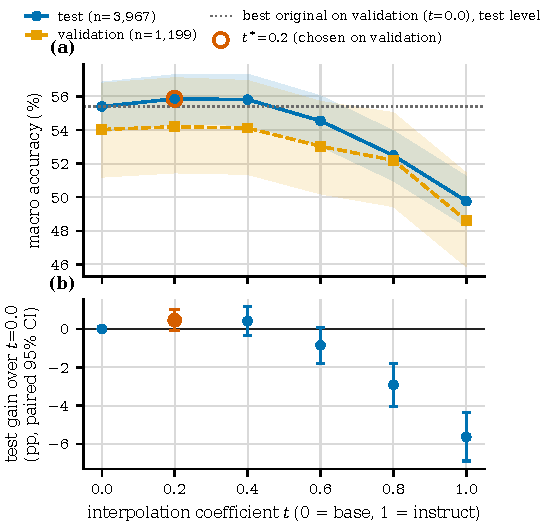
\includegraphics[width=\columnwidth]{figs/fig06_lerp_smollm2.pdf}
\caption{(a) Macro accuracy along the SmolLM2-360M base-to-instruct path: test (blue) and validation (orange, dashed) with 95\% CI bands; red ring marks the validation-selected $t^\ast$, dotted line the test level of the better original. (b) Paired test gain over the better original, with 95\% CI. Both curves are flat up to $t=0.4$ and fall beyond it.}
\label{fig:smol}
\end{figure}

\textbf{Primary result.} $t^\ast=0.2$ scores 55.86\% on test against 55.40\% for the base model: $\Delta=+0.46$ pp, 95\% CI $[-0.10,+1.02]$, $p=0.113$. The interval contains zero, so the pre-registered hypothesis is not supported; no difference was detected (no equivalence test). Against the instruct model, $t^\ast$ is better by $+6.09$ pp ($[+4.83,+7.30]$, $p<0.001$). The selection margin on validation is small: 54.20\% at $t=0.2$ against 54.12\% at $t=0.4$ and 54.03\% at $t=0$. The point estimate $+0.46$ pp is close to the Qwen result ($+0.65$ pp, $[-0.23,+1.52]$) in sign and size. Both intervals include zero, so agreement between the two nulls is not evidence of a shared positive effect. The upper limit of the 95\% CI is $+1.02$ pp over the base model on this test set.

\textbf{The instruct model is worse than the base model.} On test, instruct minus base is $-5.64$ pp (95\% CI $[-6.89,-4.35]$, $p<0.001$, below the Bonferroni threshold of 0.0083 although this contrast is descriptive); on validation it is $-5.42$ pp ($[-7.67,-3.08]$). Per task on test (descriptive; no per-task intervals computed), ARC-Easy falls from 69.2\% to 50.0\%, ARC-Challenge from 38.2\% to 34.4\%, WinoGrande from 57.8\% to 56.6\%, while HellaSwag rises from 56.4\% to 58.1\%. Merged models follow the same trend: $t=0.6$ is $-0.86$ pp ($[-1.79,+0.09]$, not distinguishable from zero) and $t=0.8$ is $-2.92$ pp ($[-4.03,-1.81]$).

\textbf{The small-$t$ merge does not inherit the deficit.} For $t\le0.4$ the paired differences against the base model are $+0.46$ and $+0.41$ pp, both intervals containing zero. The merge thus stays statistically indistinguishable from the base model while the endpoint at $t=1$ is 5.6 pp lower. This describes the path and is not a gain: the selected merge equals the base model within noise.

\textbf{The validation split is informative here.} Validation macro accuracy drops from 54.03\% ($t=0$) to 48.61\% ($t=1$), a range of 5.4 pp. The paired validation difference, instruct minus base, is $-5.42$ pp ($[-7.67,-3.08]$), so selecting on 300 items per task correctly orders the endpoints. Among $t\le0.4$ validation cannot discriminate (spread 0.17 pp), which makes the choice of $t^\ast=0.2$ over $0.4$ immaterial. This is a contrast with the Qwen pair, where the whole validation curve spans 1.1 pp.

\textbf{Exploratory contrast with Qwen.} The relative task-vector norm of Eq.~(4) is $\rho=0.0794$ for SmolLM2 and $0.0418$ for Qwen2.5-0.5B, a factor 1.9. In Qwen, instruct minus base is $+0.40$ pp on test ($[-0.62,+1.41]$) and $-1.00$ pp on validation ($[-2.75,+0.92]$), neither distinguishable from zero. This analysis was not pre-registered. The two model pairs differ in family, size, data and post-training recipe, so the data cannot separate $\rho$ from any of these factors, and two points do not define a relationship. We conjecture only that a larger weight difference leaves more room for the endpoints to differ in accuracy. We did not test this, and the result here (a worse instruct model) shows a difference in one direction only.

\textbf{What cannot be concluded.} We cannot conclude that interpolation improves SmolLM2 or fails to improve it by a fraction of a point; that the instruct model is worse in general (the benchmarks are log-likelihood multiple choice without a chat template, which may understate the instruct model); or that $\rho$ predicts merge outcomes.

\section{Discussion and Limitations}
In both families the primary hypothesis is null: neither selected merge beats the better parent beyond noise. The second family adds one different fact. Its instruct endpoint is clearly worse, the validation-selected merge lands next to the base model, and large-$t$ merges inherit a loss that the base model lacks. The practical reading is cautious: interpolation toward a worse endpoint is harmful at large $t$, not detectably harmful at small $t$, and not shown to be helpful.

\textbf{Threats to validity.} (i) Two model pairs from two families; any cross-family statement rests on $n=2$. (ii) The benchmarks are four log-likelihood multiple-choice tasks, and the instruct models are scored without chat templates, which may understate them. The per-task drop on ARC-Easy (19 pp) is large, and we did not investigate its cause. (iii) The grid has only six points with step 0.2, coarser than the eleven points used for Qwen, so a narrow optimum would be missed and the selected $t^\ast$ has less resolution. (iv) The test split is easier than validation (base: 55.4\% against 54.0\%), so we compare gains, not levels. (v) Possible contamination of benchmarks in either parent. (vi) Selecting among six candidates on one split and reporting on another limits, but does not remove, adaptive-analysis bias \cite{dwork2015adaptive}. The study also uses a single split (seed 0), one hardware platform, and a bootstrap that treats items as independent. (vii) $\rho$ is a global norm ratio, insensitive to which layers changed. (viii) All evaluations used bfloat16. The fp32 check was run only for Qwen2.5-0.5B, where validation macro accuracy shifted by $0.08$ to $0.67$~pp; SmolLM2 was not re-evaluated in fp32, so its accuracy levels may shift by a similar amount.

\section{Conclusion}
For SmolLM2-360M, validation-selected interpolation between base and instruct ($t^\ast=0.2$) is not distinguishable from the base model (no equivalence test): $+0.46$ pp, 95\% CI $[-0.10,+1.02]$ on 3{,}967 test items. The replication therefore does not support the hypothesis, as in Qwen. The new element is that SmolLM2-Instruct is 5.6 pp below the base model. The small-$t$ merge avoids that deficit but gains nothing detectable beyond the base. The relative norm of the weight difference is nearly twice that of Qwen (0.0794 against 0.0418); we report it as an exploratory contrast, not as an explanation.

\section*{Data and Code Availability}
Code, per-item caches, tables and figures are in the project repository at git tag \texttt{preprints-v1} (the commit that contains this manuscript and all scripts and caches). The tables of this paper are regenerated by \texttt{experiments/art01\_06\_tables.py} and the task-vector norms by \texttt{experiments/an\_taskvec.py} (output \texttt{results/taskvec.json}). Datasets: \texttt{allenai/ai2\_arc}, \texttt{Rowan/hellaswag}, \texttt{allenai/winogrande} (\texttt{winogrande\_xl}). Model revisions are given above and in \texttt{MANIFEST.json}. Versions: Python 3.9.6, PyTorch 2.8.0, transformers 4.57.6, numpy 1.26.4, datasets 4.5.0. The single command \texttt{./run\_everything.sh} regenerates the curves and summaries (models and data are fetched by \texttt{common/baixar.py}). The pre-registration is \texttt{experiments/PREREG.md}, written before any merge was run.

\section*{Acknowledgments}
No external funding.

\begin{thebibliography}{99}
\bibitem{allal2025smollm2} L. Ben Allal, A. Lozhkov, E. Bakouch, et al., ``SmolLM2: when smol goes big---data-centric training of a small language model,'' arXiv:2502.02737, 2025.
\bibitem{qwen2024qwen25} Qwen, A. Yang, et al., ``Qwen2.5 technical report,'' arXiv:2412.15115, 2024.
\bibitem{yang2024survey} E. Yang, L. Shen, G. Guo, et al., ``Model merging in LLMs, MLLMs, and beyond: methods, theories, applications and opportunities,'' arXiv:2408.07666, 2024.
\bibitem{li2023fusion} W. Li, Y. Peng, M. Zhang, et al., ``Deep model fusion: a survey,'' arXiv:2309.15698, 2023.
\bibitem{yadav2024scale} P. Yadav, T. Vu, J. Lai, et al., ``What matters for model merging at scale?'' arXiv:2410.03617, 2024.
\bibitem{wortsman2022wise} M. Wortsman, G. Ilharco, J. W. Kim, et al., ``Robust fine-tuning of zero-shot models,'' in \emph{Proc.\ CVPR}, 2022, arXiv:2109.01903.
\bibitem{ilharco2023taskarith} G. Ilharco, M. T. Ribeiro, M. Wortsman, et al., ``Editing models with task arithmetic,'' in \emph{Proc.\ ICLR}, 2023, arXiv:2212.04089.
\bibitem{ortiz2023tangent} G. Ortiz-Jimenez, A. Favero, and P. Frossard, ``Task arithmetic in the tangent space: improved editing of pre-trained models,'' in \emph{NeurIPS}, 2023, arXiv:2305.12827.
\bibitem{huang2023chatvector} S.-C. Huang, P.-Z. Li, Y.-C. Hsu, et al., ``Chat Vector: a simple approach to equip LLMs with instruction following and model alignment in new languages,'' in \emph{Proc.\ ACL}, 2024, arXiv:2310.04799.
\bibitem{yadav2023ties} P. Yadav, D. Tam, L. Choshen, et al., ``TIES-Merging: resolving interference when merging models,'' in \emph{NeurIPS}, 2023, arXiv:2306.01708.
\bibitem{yu2024dare} L. Yu, B. Yu, H. Yu, et al., ``Language models are Super Mario: absorbing abilities from homologous models as a free lunch,'' in \emph{Proc.\ ICML}, 2024, arXiv:2311.03099.
\bibitem{yang2024adamerging} E. Yang, Z. Wang, L. Shen, et al., ``AdaMerging: adaptive model merging for multi-task learning,'' in \emph{Proc.\ ICLR}, 2024, arXiv:2310.02575.
\bibitem{akiba2024evolutionary} T. Akiba, M. Shing, Y. Tang, et al., ``Evolutionary optimization of model merging recipes,'' \emph{Nat.\ Mach.\ Intell.}, 2025, arXiv:2403.13187.
\bibitem{huang2024lorahub} C. Huang, Q. Liu, B. Y. Lin, et al., ``LoraHub: efficient cross-task generalization via dynamic LoRA composition,'' in \emph{Proc.\ COLM}, 2024, arXiv:2307.13269.
\bibitem{sanyal2023lawa} S. Sanyal, A. Neerkaje, J. Kaddour, et al., ``Early weight averaging meets high learning rates for LLM pre-training,'' arXiv:2306.03241, 2023.
\bibitem{liu2024checkpoint} D. Liu, Z. Wang, B. Wang, et al., ``Checkpoint merging via Bayesian optimization in LLM pretraining,'' arXiv:2403.19390, 2024.
\bibitem{wortsman2022soups} M. Wortsman, G. Ilharco, S. Y. Gadre, et al., ``Model soups: averaging weights of multiple fine-tuned models improves accuracy without increasing inference time,'' in \emph{Proc.\ ICML}, 2022, arXiv:2203.05482.
\bibitem{goddard2024mergekit} C. Goddard, S. Siriwardhana, M. Ehghaghi, et al., ``Arcee's MergeKit: a toolkit for merging large language models,'' arXiv:2403.13257, 2024.
\bibitem{clark2018arc} P. Clark, I. Cowhey, O. Etzioni, et al., ``Think you have solved question answering? Try ARC, the AI2 Reasoning Challenge,'' arXiv:1803.05457, 2018.
\bibitem{zellers2019hellaswag} R. Zellers, A. Holtzman, Y. Bisk, et al., ``HellaSwag: can a machine really finish your sentence?'' in \emph{Proc.\ ACL}, 2019, arXiv:1905.07830.
\bibitem{sakaguchi2020winogrande} K. Sakaguchi, R. Le Bras, C. Bhagavatula, et al., ``WinoGrande: an adversarial Winograd schema challenge at scale,'' in \emph{AAAI}, 2020, arXiv:1907.10641.
\bibitem{gao2023harness} L. Gao et al., ``EleutherAI/lm-evaluation-harness,'' Zenodo, doi:10.5281/zenodo.10256836.
\bibitem{miller2024errorbars} E. Miller, ``Adding error bars to evals: a statistical approach to language model evaluations,'' arXiv:2411.00640, 2024.
\bibitem{dwork2015adaptive} C. Dwork, V. Feldman, M. Hardt, et al., ``Preserving statistical validity in adaptive data analysis,'' arXiv:1411.2664, 2014.
\bibitem{efron1979bootstrap} B. Efron, ``Bootstrap methods: another look at the jackknife,'' \emph{Ann. Statist.}, vol.~7, no.~1, 1979, doi:10.1214/aos/1176344552.
\bibitem{santos2026modelmergingfo} D. F. Santos, ``Model Merging for Capability Composition: A Technical Note,'' Zenodo, 2026, doi:10.5281/zenodo.21610555.
\bibitem{santos2026collapseresist} D. F. Santos, ``Collapse-Resistant Joint-Embedding Predictive Architectures: A Controlled Comparison of SIGReg, VICReg, and EMA,'' Zenodo, v2, 2026, doi:10.5281/zenodo.24223364.
\bibitem{santos2026knowledgedisti} D. F. Santos, ``Knowledge Distillation and Self-Distillation for Language Models,'' Zenodo, 2026, doi:10.5281/zenodo.21610100.
\bibitem{santos2026parametereffic} D. F. Santos, ``Parameter-Efficient Fine-Tuning: LoRA, QLoRA, and DoRA,'' Zenodo, 2026, doi:10.5281/zenodo.21610033.
\bibitem{santos2026mixtureofexper} D. F. Santos, ``Mixture-of-Experts Training and Sparse Upcycling,'' Zenodo, 2026, doi:10.5281/zenodo.21610062.
\bibitem{santos2026curriculumlear} D. F. Santos, ``Curriculum Learning and Data-Efficient Pretraining: A Technical Note,'' Zenodo, 2026, doi:10.5281/zenodo.21610595.
\bibitem{santos2026syntheticdatag} D. F. Santos, ``Synthetic Data Generation and Self-Improvement: A Technical Note,'' Zenodo, 2026, doi:10.5281/zenodo.21610525.
\bibitem{santos2026directpreferen} D. F. Santos, ``Direct Preference Optimization (DPO): A Technical Note,'' Zenodo, 2026, doi:10.5281/zenodo.21609911.
\bibitem{santos2026rlaifandconsti} D. F. Santos, ``RLAIF and Constitutional AI: A Technical Note,'' Zenodo, 2026, doi:10.5281/zenodo.21610280.
\bibitem{santos2026reinforcementl} D. F. Santos, ``Reinforcement Learning with Verifiable Rewards (RLVR) and GRPO for Reasoning,'' Zenodo, 2026, doi:10.5281/zenodo.21609980.
\end{thebibliography}

\end{document}
